\clearpage
\subsectionold{MSVC + \olly}
\myindex{\olly}

Загрузим наш пример в \olly и установим точку останова на функции \comp{}.
Как значения сравниваются, мы можем увидеть во время самого первого вызова \comp{}:

\begin{figure}[H]
\centering
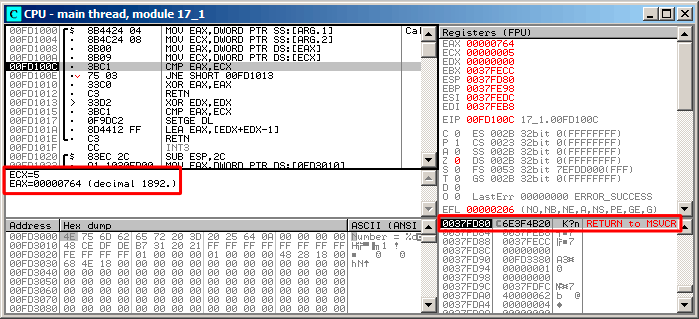
\includegraphics[scale=\FigScale]{patterns/18_pointers_to_functions/olly1.png}
\caption{\olly: первый вызов \comp}
\label{fig:qsort_olly1}
\end{figure}

Для удобства, \olly показывает сравниваемые значения в окне под окном кода.
Мы можем так же увидеть, что \ac{SP} указывает на \ac{RA} где находится место в функции \qsort (на самом деле, находится в \TT{MSVCR100.DLL}).

\clearpage
Трассируя (F8) до инструкции \TT{RETN} и нажав F8 еще один раз, мы возвращаемся в функцию \qsort:

\begin{figure}[H]
\centering
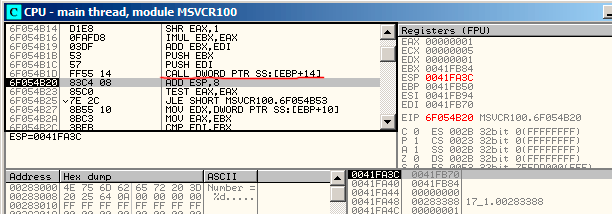
\includegraphics[scale=\FigScale]{patterns/18_pointers_to_functions/olly2.png}
\caption{\olly: код в \qsort сразу после вызова \comp}
\label{fig:qsort_olly2}
\end{figure}

Это был вызов функции сравнения.

\clearpage
Вот также скриншот момента второго вызова функции \comp{}---теперь сравниваемые значения другие:

\begin{figure}[H]
\centering
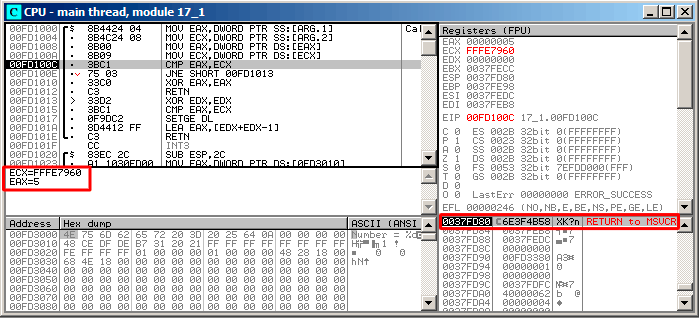
\includegraphics[scale=\FigScale]{patterns/18_pointers_to_functions/olly3.png}
\caption{\olly: второй вызов \comp}
\label{fig:qsort_olly3}
\end{figure}
